\documentclass[11pt]{article}
\usepackage[margin=1in]{geometry}
\usepackage{booktabs}
\usepackage{graphicx}
\usepackage{adjustbox}
\usepackage{float}
\usepackage{hyperref}
\usepackage{caption}
\usepackage{setspace}
\usepackage{siunitx}
\usepackage{amsmath}

\begin{document}
\singlespacing

\section*{Part 4: Results and Methods}

\subsection*{Data and scope}
We study PJM day-ahead LMP and (separately) load forecasts joined to NOAA ISD hourly weather at station locations mapped to each pricing node. The current correlation export contains \num{1974} node--year--variable records (weather vs.\ LMP, Pearson $r$) across \num{76} nodes and \num{24} balancing-area zones; calendar years \num{2021}--\num{2025} appear in the series. Period tags in code treat \texttt{earlyAI} as the \num{2021} slice and \texttt{recentAI} as \num{2022}--\num{2025}, so year-to-year trend plots partially confound calendar year with the period definition.

\subsection*{Methods}

\paragraph{Weather merge and features.}
For each node and year, PJM hourly records were aligned to UTC and merged to NOAA ``global hourly'' fields using nearest-time matching (\texttt{merge\_asof}, \SI{30}{minute} tolerance). Sentinels were nulled; temperature, dew point, pressure, wind, and precipitation were converted to physical units. Cooling and heating degree hours (base \SI{18}{\celsius}) and relative humidity (Magnus form) were computed in \texttt{scripts/build\_analysis\_exports.py} and \texttt{scripts/train\_rq2\_models.py}.

\paragraph{RQ1 (associational).}
For each node, year, weather variable, and target (day-ahead LMP or load), we computed Pearson correlation between the merged weather series and the target. Rows carry a DC vs.\ non-DC bucket derived from explainable node scoring (\texttt{scripts/export\_pjm\_metadata.py}) propagated into \texttt{data/exports/correlations\_by\_region\_period.json}.

\paragraph{RQ2 (predictive).}
We featurized merged hourly panels per node--year (weather signals plus calendar indicators where implemented), imposed a chronological evaluation split with held-out test years starting at \num{2024}, median-imputed missing values, standardized inputs for linear learners, and trained six regressors per configuration: ordinary least squares, Ridge ($\alpha{=}1$), Lasso ($\alpha{=}0.001$), RandomForest (\num{90} trees), GradientBoosting, and ExtraTrees (\num{100} trees). Metrics were computed on the held-out portion (RMSE, MAE, $R^2$); weather-only $\mathrm{nRMSE} = \mathrm{RMSE}/\lvert\bar{y}\rvert$ when the held-out target mean $\bar{y}$ is available. The training entry point is \texttt{python scripts/train\_rq2\_models.py} (flags for year range, node cap, and data volume). Results are written to \texttt{data/exports/model\_performance.json} and consumed by the React app after \texttt{npm run sync:data}.

\paragraph{Between-group summaries.}
\texttt{scripts/build\_hypothesis\_exports.py} aggregates node-level absolute correlations for RQ1 and weather-only $n$RMSE rows for RQ2; it computes bootstrap \num{95}\% confidence intervals for the DC-minus-non-DC mean contrast (when minimum group sizes are met), two-sided permutation $p$-values (\num{3000} draws, seed \num{42}), Cohen's $d$, and marks descriptive-only outputs when gates fail.

\paragraph{Figures (trends vs.\ bucket contrasts).}
Figures~\ref{fig:dcbucket}--\ref{fig:linebucket} regenerate from \path{correlations_by_region_period.json} via \path{docs/generate_report_figures.py}. DC-aware distribution and bootstrap panels (Figs.~\ref{fig:rq1dist}--\ref{fig:rq2inf}) come from \path{docs/generate_rq_research_figures.py}, using \path{nodes.json}, correlations, \path{model_performance.json}, and \path{hypothesis_tests.json}.

\subsection*{Results}

\begin{figure}[H]
\centering
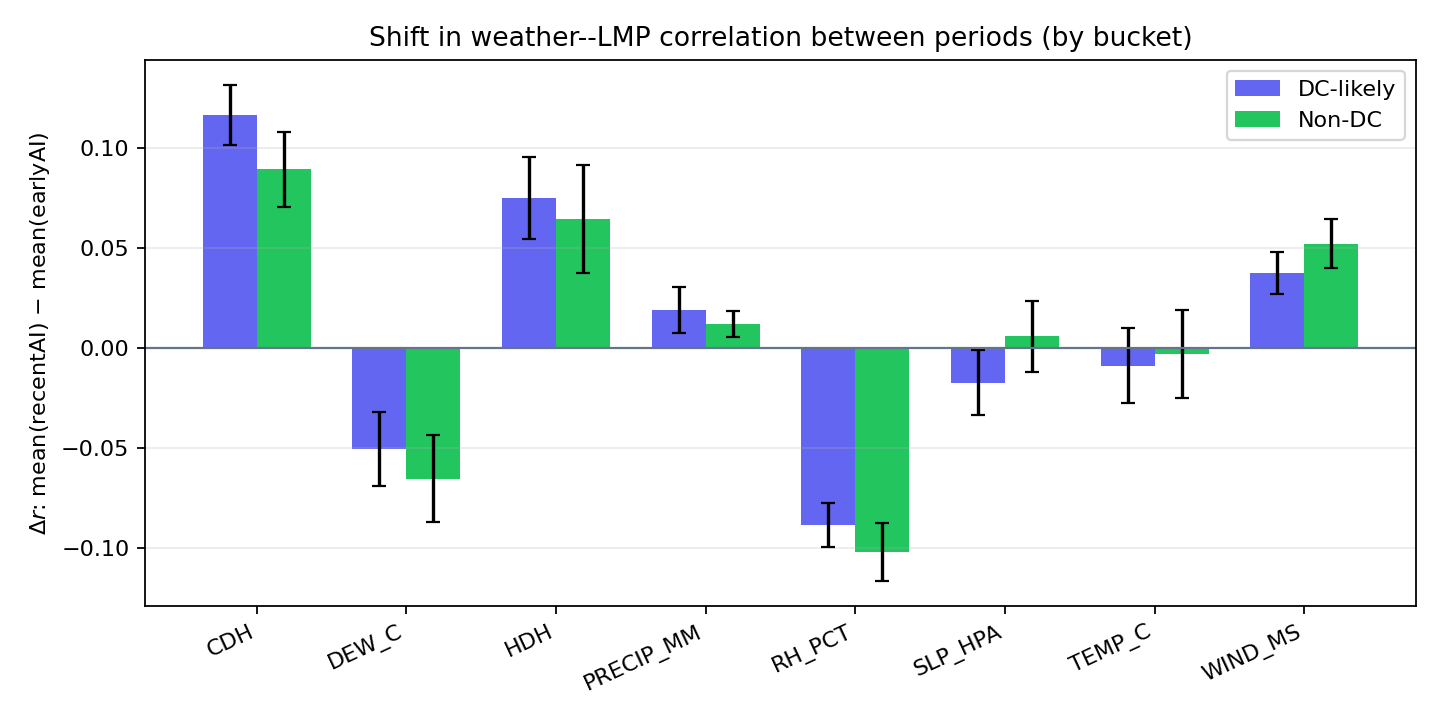
\includegraphics[width=0.82\textwidth]{heavy_vs_nonheavy_shift.png}
\caption{Fig.\ 1: Mean shift in weather--LMP correlation between \texttt{recentAI} (\num{2022}--\num{2025}) and \texttt{earlyAI} (\num{2021}), by DC-likelihood bucket and weather variable; error bars reflect independent SEM propagation across periods.}
\label{fig:dcbucket}
\end{figure}

\begin{figure}[H]
\centering
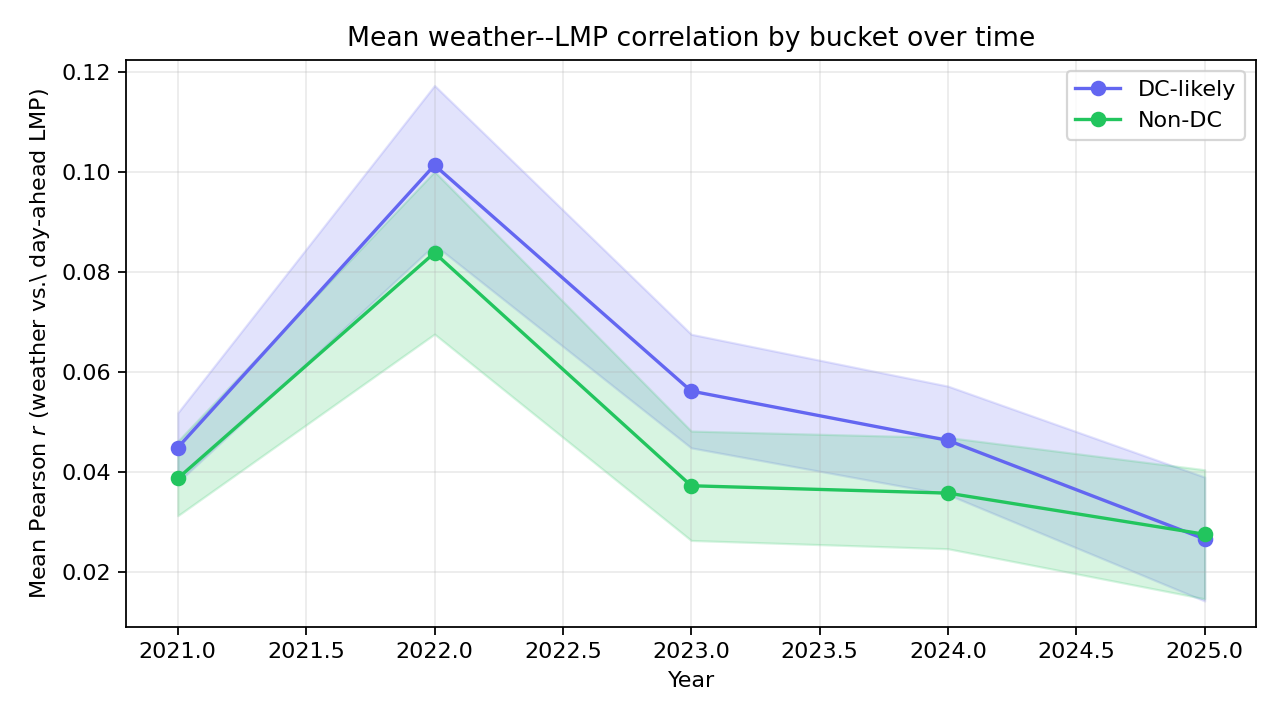
\includegraphics[width=0.82\textwidth]{avg_corr_by_bucket_over_time.png}
\caption{Fig.\ 2: Mean Pearson $r$ (weather vs.\ LMP) by calendar year and bucket; shaded bands are $\pm 1$\,SEM within each year$\times$bucket cell.}
\label{fig:linebucket}
\end{figure}

\noindent
Figures~\ref{fig:dcbucket}--\ref{fig:linebucket} summarize variable-level associational contrasts over time (RQ1 context); they compress many nodes into bucket means.

\paragraph*{RQ1 and RQ2: distributions and mean-difference uncertainty.}
Figures~\ref{fig:rq1dist}--\ref{fig:rq2inf} emphasize spread, \(n\), and uncertainty rather than bar-chart means alone. Distribution panels are \emph{descriptive}; CI plots show point estimate and bootstrap interval only (\emph{plot-only}, no embedded prose). All contrast definitions (which mean is differenced), sample sizes, numerical CI bounds, permutation \(p\)-values, and node-level vs.\ evaluation-row distinctions for RQ2 appear in this subsection's captions and Table~\ref{tab:hyp}, not duplicated on the PNGs.

\begin{figure}[H]
\centering
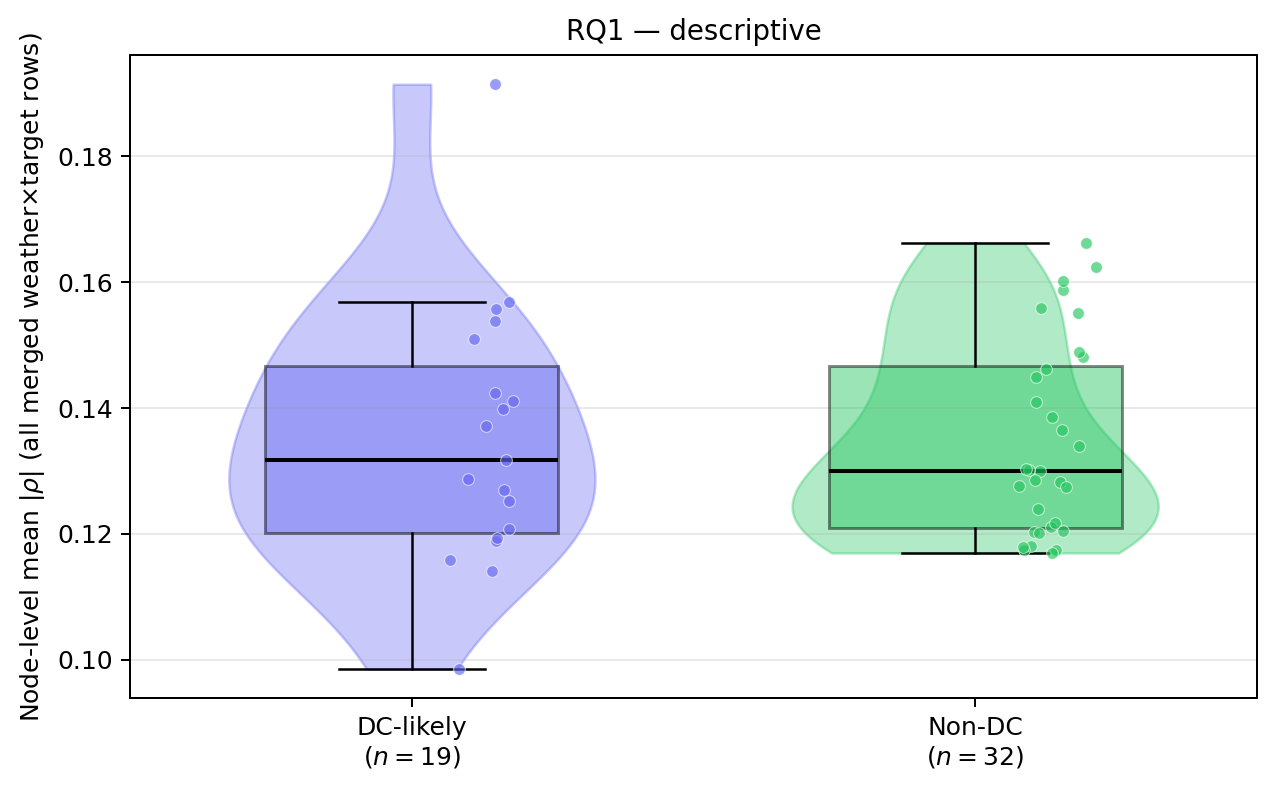
\includegraphics[width=0.88\textwidth]{rq1_distribution_node_abs_corr.png}
\caption{\textbf{Descriptive (RQ1).} Node-level mean absolute Pearson correlation (all merged weather$\times$target rows per node), by DC-likelihood bucket. Violin shading, box quartiles, and jittered points show overlap and tails; axis labels include group \(n\).}
\label{fig:rq1dist}
\end{figure}

\begin{figure}[H]
\centering
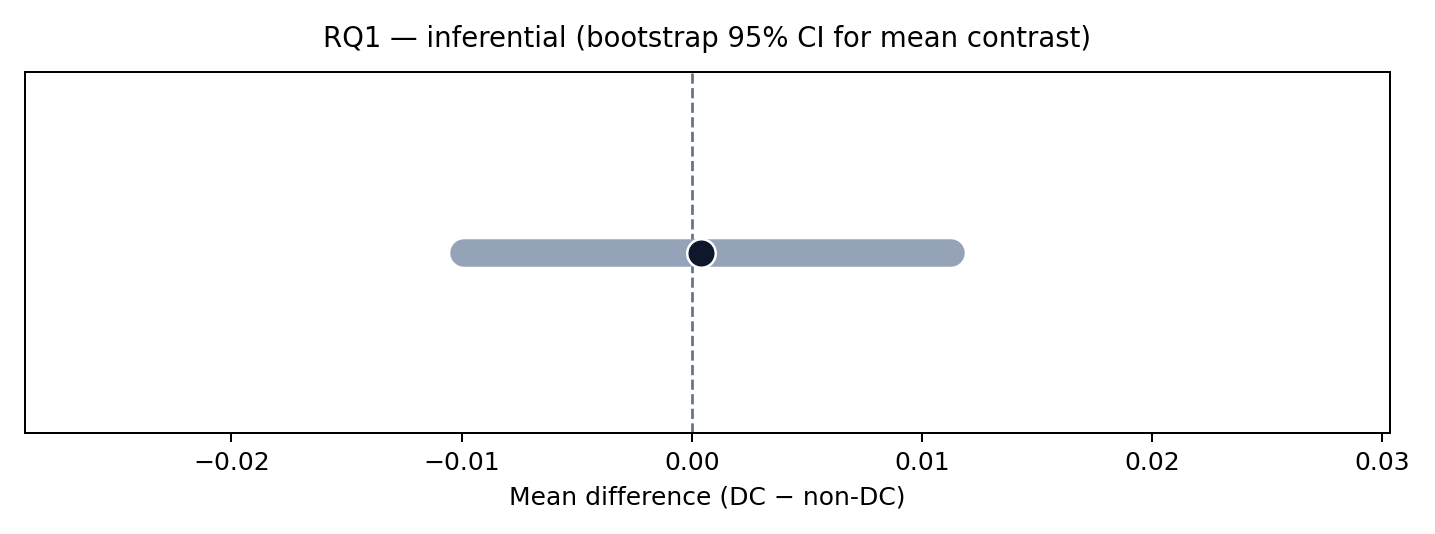
\includegraphics[width=0.88\textwidth]{rq1_inferential_mean_diff_ci.png}
\caption{\textbf{Inferential (RQ1).} Bootstrap \num{95}\% CI for the difference of \emph{group means} of node-level mean \(|\rho|\) (DC $-$ non-DC), aligned with \texttt{hypothesis\_tests.json}. Interval crossing \num{0} is consistent with no detectable mean shift at this precision; significance follows Table~\ref{tab:hyp}, not the graphic alone.}
\label{fig:rq1inf}
\end{figure}

\noindent
For RQ1, Figs.~\ref{fig:rq1dist}--\ref{fig:rq1inf} support the same story as Table~\ref{tab:hyp}: distributions largely overlap and the inferential CI for the mean difference straddles zero (\(p=\num{0.945}\)).

\begin{figure}[H]
\centering
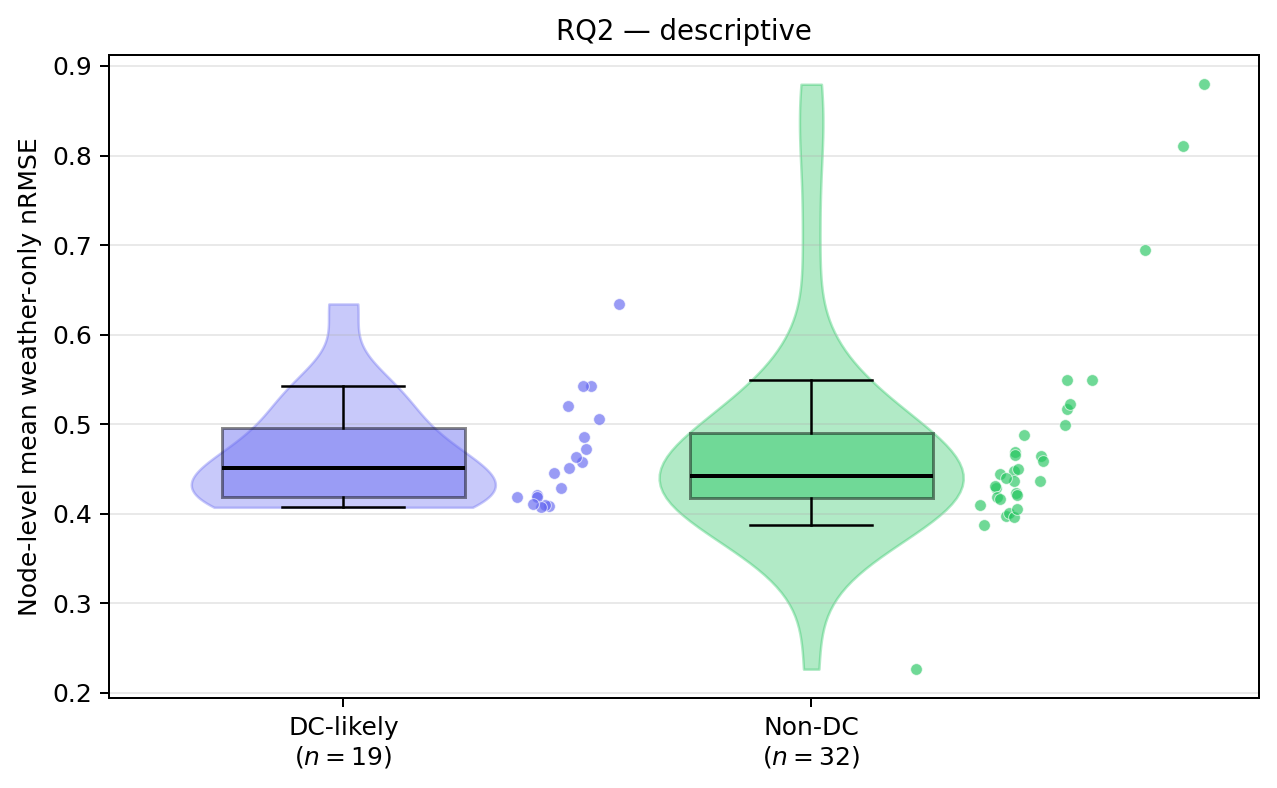
\includegraphics[width=0.88\textwidth]{rq2_distribution_node_weather_only_metric.png}
\caption{\textbf{Descriptive (RQ2).} Node-level mean weather-only error (per-node average across exported evaluation rows; \(n\)RMSE when available so scale is comparable across nodes). High dispersion reflects model and period heterogeneity within buckets.}
\label{fig:rq2dist}
\end{figure}

\begin{figure}[H]
\centering
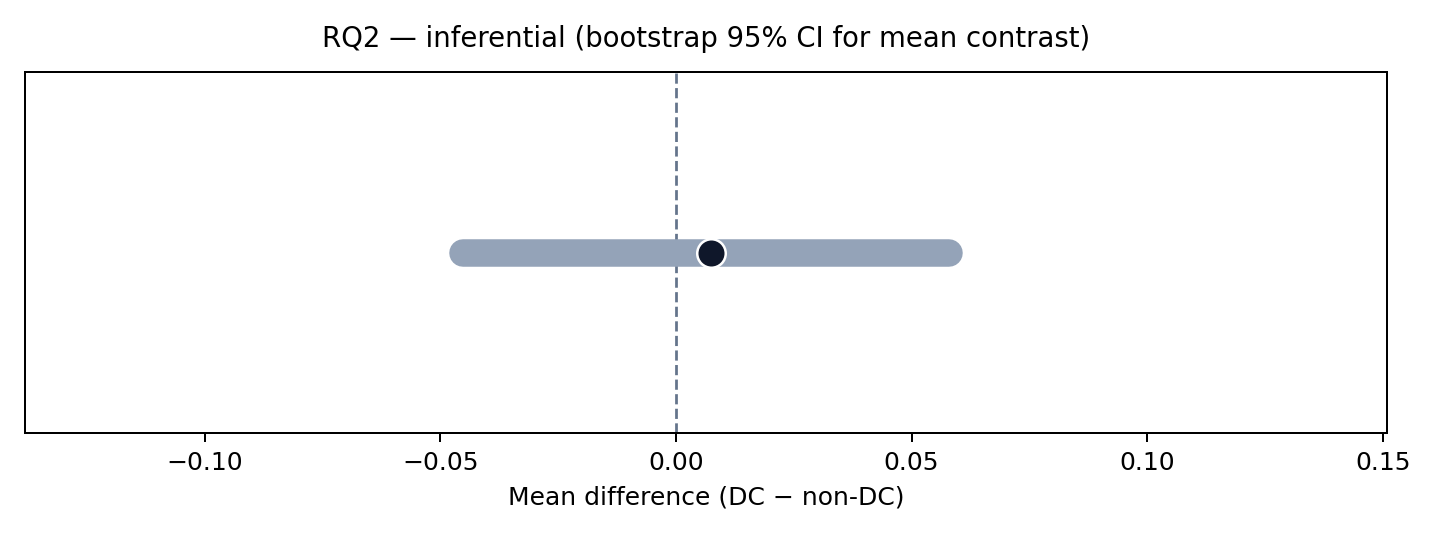
\includegraphics[width=0.88\textwidth]{rq2_inferential_mean_diff_ci.png}
\caption{\textbf{Inferential (RQ2).} Bootstrap \num{95}\% CI for DC $-$ non-DC mean weather-only \(n\)RMSE using \emph{evaluation rows} (possibly multiple per node), as in the hypothesis export. Descriptive Fig.~\ref{fig:rq2dist} uses node-level means for clarity; interpret inferential claims from Table~\ref{tab:hyp} and this panel.}
\label{fig:rq2inf}
\end{figure}

\noindent
For RQ2, Fig.~\ref{fig:rq2dist} shows substantial within-bucket spread; Fig.~\ref{fig:rq2inf} and Table~\ref{tab:hyp} show a small mean contrast with CI spanning zero (\(p=\num{0.791}\)), so we do not claim a reliable accuracy gap between buckets under this specification.

\begin{table}[H]
\centering
\caption{Hypothesis-export contrasts at $\alpha = 0.05$ (from \texttt{hypothesis\_tests.json}). CI = bootstrap mean difference DC $-$ non-DC.}
\label{tab:hyp}
\adjustbox{max width=\linewidth}{%
\begin{tabular}{@{}lcccc@{}}
\toprule
RQ & Metric & $n$ DC / non-DC & Means (DC; non-DC) & CI / $p$ / Cohen's $d$ \\
\midrule
1 & Mean $|r|$ per node & \num{19}; \num{32} & \num{0.135}; \num{0.135} & $[-0.010,\,0.011]$; $p{=}0.945$; $d{=}0.022$ \\
2 & Weather-only $n$RMSE (rows) & \num{324}; \num{270} & \num{0.465}; \num{0.457} & $[-0.045,\,0.058]$; $p{=}0.791$; $d{=}0.023$ \\
\bottomrule
\end{tabular}%
}
\end{table}

\noindent
\textbf{Descriptive comparison (means only).}
DC-likely nodes register a slightly higher mean absolute weather correlation than non-DC nodes (mean difference \(\approx\num{0.0004}\), relative \(\approx\num{0.3}\,\%\); Table~\ref{tab:hyp}).
For weather-only forecasts, mean \(n\)RMSE is modestly higher in the DC-likely bucket (\(\approx\num{0.465}\) vs.\ \(\approx\num{0.457}\)): that group shows somewhat larger normalized error on average (\(\approx\num{1.6}\,\%\) relative gap), i.e.\ slightly worse aggregate weather-only fit than non-DC nodes in this dataset slice.
These sentences summarize central tendencies only and avoid significance thresholds or \(p\)-values.

\noindent
Table~\ref{tab:hyp} matches Figs.~\ref{fig:rq1inf} and~\ref{fig:rq2inf}: neither mean contrast is significant at $\alpha=\num{0.05}$ (RQ1 $p=\num{0.945}$, RQ2 $p=\num{0.791}$); Cohen's $d$ is negligible in both cases.

The React dashboard (\texttt{OverviewPage}) mirrors these panels (box + jitter + CI cards; Models page: filters by target and learner). Inferential captions follow Table~\ref{tab:hyp}.

\subsection*{Reproducibility}
\begin{itemize}
  \item \textbf{Repository:} \url{https://github.com/jaiparmar940/energy-weather-app}
  \item \textbf{Trend figures (Fig.~\ref{fig:dcbucket}--\ref{fig:linebucket}):} \path{python docs/generate_report_figures.py}
  \item \textbf{RQ distribution / CI figures (Fig.~\ref{fig:rq1dist}--\ref{fig:rq2inf}):} \path{python docs/generate_rq_research_figures.py}
  \item \textbf{Model and hypothesis exports:} \path{python scripts/train_rq2_models.py}; then \path{python scripts/build_hypothesis_exports.py}; then \path{npm run sync:data}.
\end{itemize}

\end{document}
